%%%%%%%%%%%%%%%%%%%%%%%%%%%%%%%%%%%%%%%%%%%%%%%%%%%%%%%%%%%%%%%%%%%%%%%%%%%%%%%%
%2345678901234567890123456789012345678901234567890123456789012345678901234567890
%        1         2         3         4         5         6         7         8

\documentclass[letterpaper, 10 pt, conference]{ieeeconf}  % Comment this line out if you need a4paper

%\documentclass[a4paper, 10pt, conference]{ieeeconf}      % Use this line for a4 paper

\IEEEoverridecommandlockouts                              % This command is only needed if 
                                                          % you want to use the \thanks command

\overrideIEEEmargins                                      % Needed to meet printer requirements.

% See the \addtolength command later in the file to balance the column lengths
% on the last page of the document

% The following packages can be found on http:\\www.ctan.org
\usepackage{graphics} % for pdf, bitmapped graphics files
\usepackage{epsfig} % for postscript graphics files
\usepackage{mathptmx} % assumes new font selection scheme installed
\usepackage{times} % assumes new font selection scheme installed
\usepackage{amsmath} % assumes amsmath package installed
\usepackage{amssymb}  % assumes amsmath package installed

\title{\LARGE \bf
ESE650 Project 1: Automatic Detection of Red Barrels
}


\author{Achille Verheye% <-this % stops a space
}


\begin{document}



\maketitle
\thispagestyle{empty}
\pagestyle{empty}


%%%%%%%%%%%%%%%%%%%%%%%%%%%%%%%%%%%%%%%%%%%%%%%%%%%%%%%%%%%%%%%%%%%%%%%%%%%%%%%%
\begin{abstract}

This report describes the algorithm for fast automatic detection of red barrels in images using Gaussian models, computer vision techniques, and shape analysis. The algorithm works in most cases, can detect multiple barrels, and estimates the distance to the barrel using a linear regression model.

\end{abstract}


%%%%%%%%%%%%%%%%%%%%%%%%%%%%%%%%%%%%%%%%%%%%%%%%%%%%%%%%%%%%%%%%%%%%%%%%%%%%%%%%
\section{INTRODUCTION}

Detecting objects in images and estimating the distance from the camera is useful for robotics applications such as grasping and path planning. Humans are far better and faster than computers at distinguishing and labeling objects in various lighting conditions and with partial occlusion. Detecting simple, convex objects such as red barrels can prove to be untrivial for computers, considering the very short learning time, simplicity of the model, the limited computing resources, and the lack of stereo vision. Wrong labeling can occur when lighting conditions are suboptimal, the object is partially occluded, or other objects similar in shape and color are present. The algorithm can prove to be useful in more constant situations to locate a large number of objects in a scene. In a factory, a fast and lightweight algorithm can be used to locate and estimate pose of hundreds of items over a short period of time with few mistakes.

\section{TECHNICAL APPROACH}

\subsection{Training the Color Models}
The given data set consists of 50 images taken with the same camera and of the same dimensions. This set is then split into a training set (40 images) and a validation set (10).

First, a Gaussian color model is trained on a set of labeled training images. A user is prompted to select regions in an image that contain certain colors. Specifically, a color model is trained for red barrels, and several other color models can be trained that represent colors that are close to, but not the red of the barrel, such as brown, yellow, red from bricks, etc. Regions selected by the user are analyzed in a color space that is optimal for distinguishing colors. Particularly, color spaces that separate luma from chroma such as the HSV color space are a good fit for this problem. A single Gaussian was trained on each color model using Expectation Maximization, which determines optimal parameters for the normal distribution that models the color. The normal distribution is described by a mean and a variance and are calculated as

\begin{align*}
\mu^* &= \frac{1}{|D_{\alpha}|} \sum_{x\in D_{\alpha}} x \\
\Sigma^* &= \frac{1}{|D_{\alpha}|} \sum_{x\in D_{\alpha}} (x-\mu)(x-\mu)^T
\end{align*}
where $D_{\alpha}$ represents the set of all pixels contained in all regions selected by the user for a specific color. Each pixel has three values (H,S,V) and thus the optimal mean is a vector of length three whereas the covariance matrix is of size 3x3.

Table \ref{mu} shows the trained colors and the corresponding mean values.
\begin{table}[h]
\caption{Trained color models}
\label{mu}
\begin{center}
\begin{tabular}{|c|c|}
\hline
Color & $\mu$(H,S,V)\\
\hline
barrel red & 122, 194, 160\\
\hline
other red & 110, 132, 184\\
\hline
brown & 105, 130, 119\\
\hline
\end{tabular}
\end{center}
\end{table}

These values are then stored to file along with the color they represent for use when evaluating the algorithm on the validation set.

\subsection{Finding Barrels}

\subsubsection{Segmentation: Predicting pixel color using Likelihoods}
A new image is loaded in a script and a 'RedBarrelDetector' Python instance is initialized. This operation loads the color models trained before. The image is converted to the HSV color space just as the training images were. The first step in the detection process is the labeling of the individual pixels. This is done by computing the likelihoods that a pixel corresponds to each color model. These likelihoods represent approximations of the probability that the pixel originates from the normal distribution of a color model. We can see this by examining Bayes' rule:
\begin{equation} \label{bayes}
p(W|X) = \frac{p(X|W)p(W)}{p(X)}
\end{equation}
The term on the left hand side of (\ref{bayes}) represents the posterior probability mass function (pmf), which can loosely be interpreted as a measure of a probability that a given pixel belongs to a color model. On the right hand side, the numerator is comprised of the data likelihood $p(X|W)$ and the prior pmf $p(W)$. The denominator $p(X)$ normalizes and as it is constant, it doesn't affect the relative influence between various color models. The prior does vary between color models but is assumed a constant as well. It can be trained on the given data set, but one can intuitively see that it would negatively affect the result in unseen cases, such as when a scene has many more red barrels than in the training set. Hence, the likelihood is a good descriptor of the actual pmf. It is calculated as in (\ref{likelihood}).
\begin{equation} \label{likelihood}
\phi(x;\mu,\Sigma) = \frac{1}{\sqrt{(2\pi)^n det(\Sigma)}} exp \left(-\frac{1}{2}(x-\mu)^T \Sigma^{-1}(x-\mu)\right)
\end{equation}
After evaluating the likelihoods as described above, each pixel is assigned the color that corresponds to the maximum likelihood for that pixel. Finally, a binary image is created that represents all pixels where the color 'barrel red' was most likely. This image is stored in the RedBarrelDetector instance for further analysis. An example can be found in the top right section of Fig. \ref{resultfig}

\subsubsection{Translating Segmentation into Barrels}
The result from using the Gaussian model segmentation can contain false positives and false negatives; pixels that are classified as barrel red while they are not and pixels that are classified as some other color while they are part of the barrel. Furthermore, partial occlusion forms another challenge to this vision problem. It is obvious that eliminating false positives using naive shape analysis does not work in these cases. The approach as outlined is based on the idea that it is more useful in practice to bias the trade-off between false positives and false negatives towards the false positives; that is, prefer detection of objects that are not red barrels in reality as opposed to being conservative and missing out actual barrels. The reason is that in practice, multiple sequential images of the scene are taken and the false positives can be filtered out more efficiently. This decision depends on the specific use case.

Most of the operations performed on the segmented image are based on contours found using the OpenCV package in Python. However, before finding contours, closing and opening is performed on the binary image. Informally, the former removes small blobs of pixels that are likely artifacts, the latter closes convex regions. These operations limit the number of contours present and thus speed up the process.

Next, area is calculated for each contour as the number of pixels enclosed. Contours that have an area that is smaller than 2\% of the largest area found in the image are discarded too further limit the possible barrels. This operation may remove barrels that are very far in the scene, but it is argued that those barrels are less important than the ones in the front and are more likely to just be artifacts. The remaining contours are compared pairwise both in distance and in area with the idea that contours that are close are probable to be part of the same barrel. The weighted distance was calculated as in (\ref{weighted_dist}).
\begin{align} \label{weighted_dist}
D_{centroids} &= \sqrt{(\vec{c_1}-\vec{c_2})^2} \\
D_{weigthed} &= \frac{D_{centroids}^3}{area_1 + area_2}
\end{align}

with $\vec{c_i}$ the centroid of a contour. Two contours are considered to be part of the same physical structure when this weighted distance was smaller than $300$, empirically determined from the validation set. In that case, the convex hull of the two contours is calculated and thus joined. Minimally enclosing rectangles are then found using OpenCV's built-in functions and stored to the RedBarrelDetector instance.

\subsection{Training Distance}

The given training set specifies the distances to each barrel in the image. A linear regression model relates these distances to the area computed for each barrel using the trained RedBarrelDetector. Intuitively, it makes sense that the farther away the barrel, the smaller its area in the image. When a new image is tested, the area of its barrel is fed to the trained regressor which then estimates the distance.

\section{RESULTS}
\subsection{Validation Set}
Figures (\ref{resultfig}), (\ref{resultfig-occluded}), and (\ref{resultfig-fail}) show samples of resulting detection along with the result from initial segmentation and using computer vision techniques to detect the barrels. Results on a validation set of 10 images were as in Table \ref{resultsvalidation}. One image contained two barrels. 

\begin{table}[h]
\caption{Detection results on 10 images with a total of 11 barrels. number of objects classified as barrel = 12}
\label{resultsvalidation}
\begin{center}
\begin{tabular}{|c|c|}
\hline
detected object & \# occurences\\
\hline
full barrel & 6\\
\hline
large part of barrel & 3\\
\hline
small part of barrel & 0\\
\hline
barrel combined with non-barrel & 2\\
\hline
non-barrel & 1\\
\hline
\end{tabular}
\end{center}
\end{table}

   \begin{figure}[thpb]
      \centering
      \framebox{\parbox{3in}{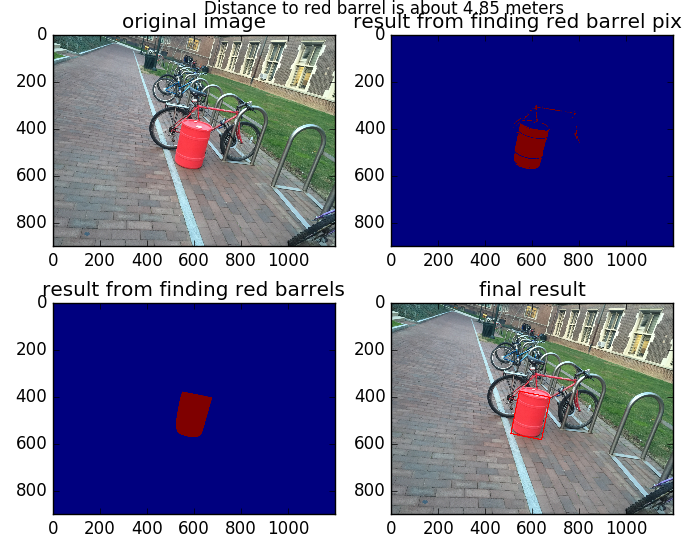
\includegraphics[scale=0.53]{result4}}}
      
      \caption{Result of a successful detection of the red barrel. A rectangular section is drawn arond the barrel in the bottom right.}
      \label{resultfig}
   \end{figure}


   \begin{figure}[thpb]
      \centering
      \framebox{\parbox{3in}{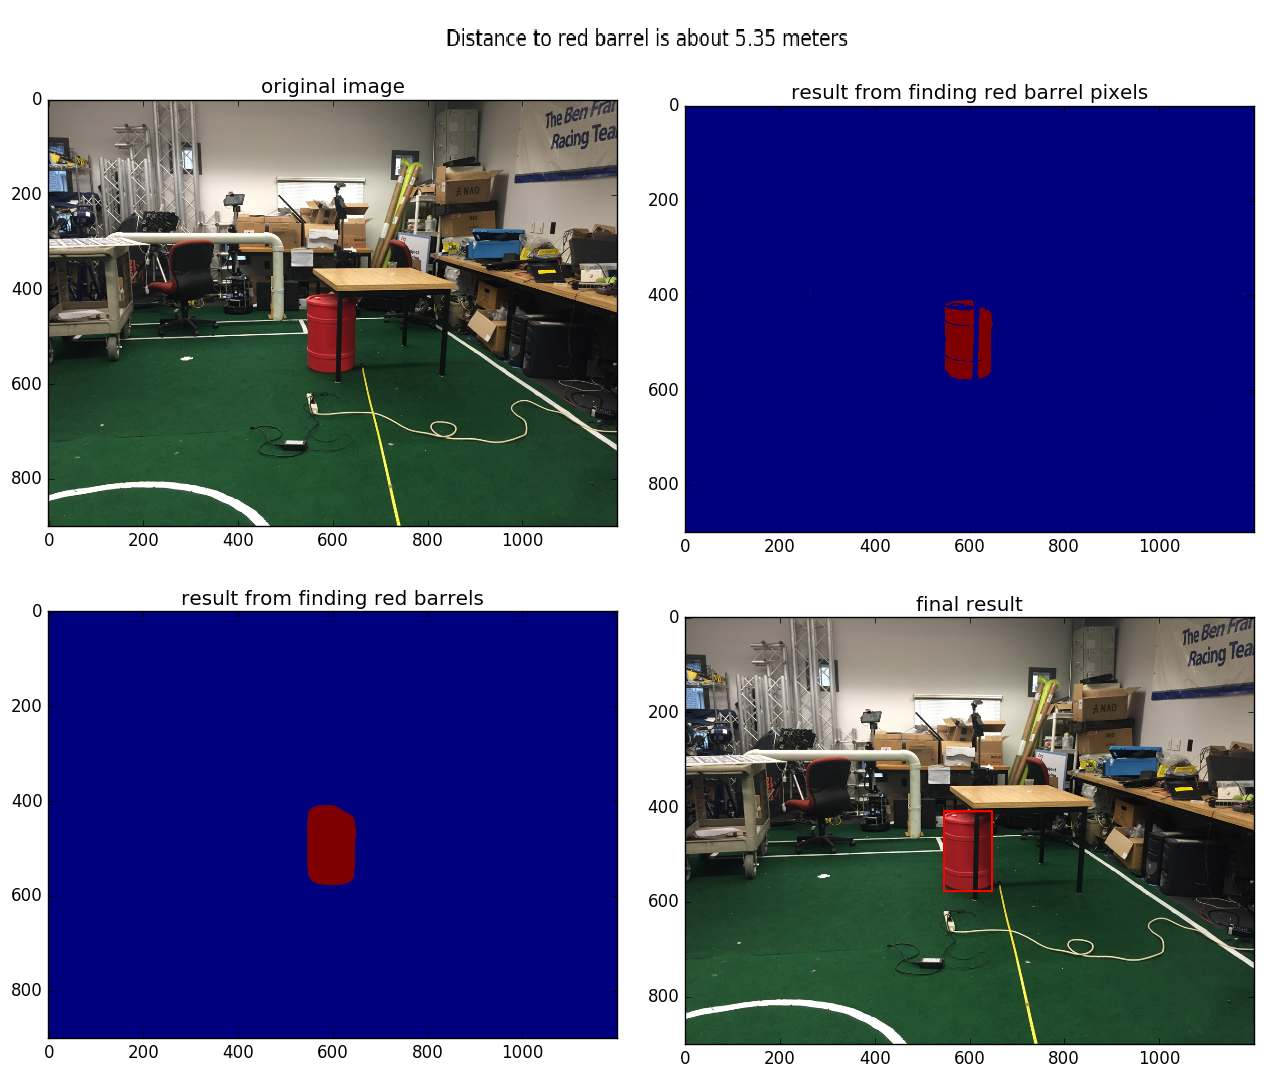
\includegraphics[scale=0.28]{result5}}}
      
      \caption{Result of a successful detection of a partially occluded red barrel. Combining contours re-unites nearby parts (bottom-right).}
      \label{resultfig-occluded}
   \end{figure}
   
   
   \begin{figure}[thpb]
      \centering
      \framebox{\parbox{3in}{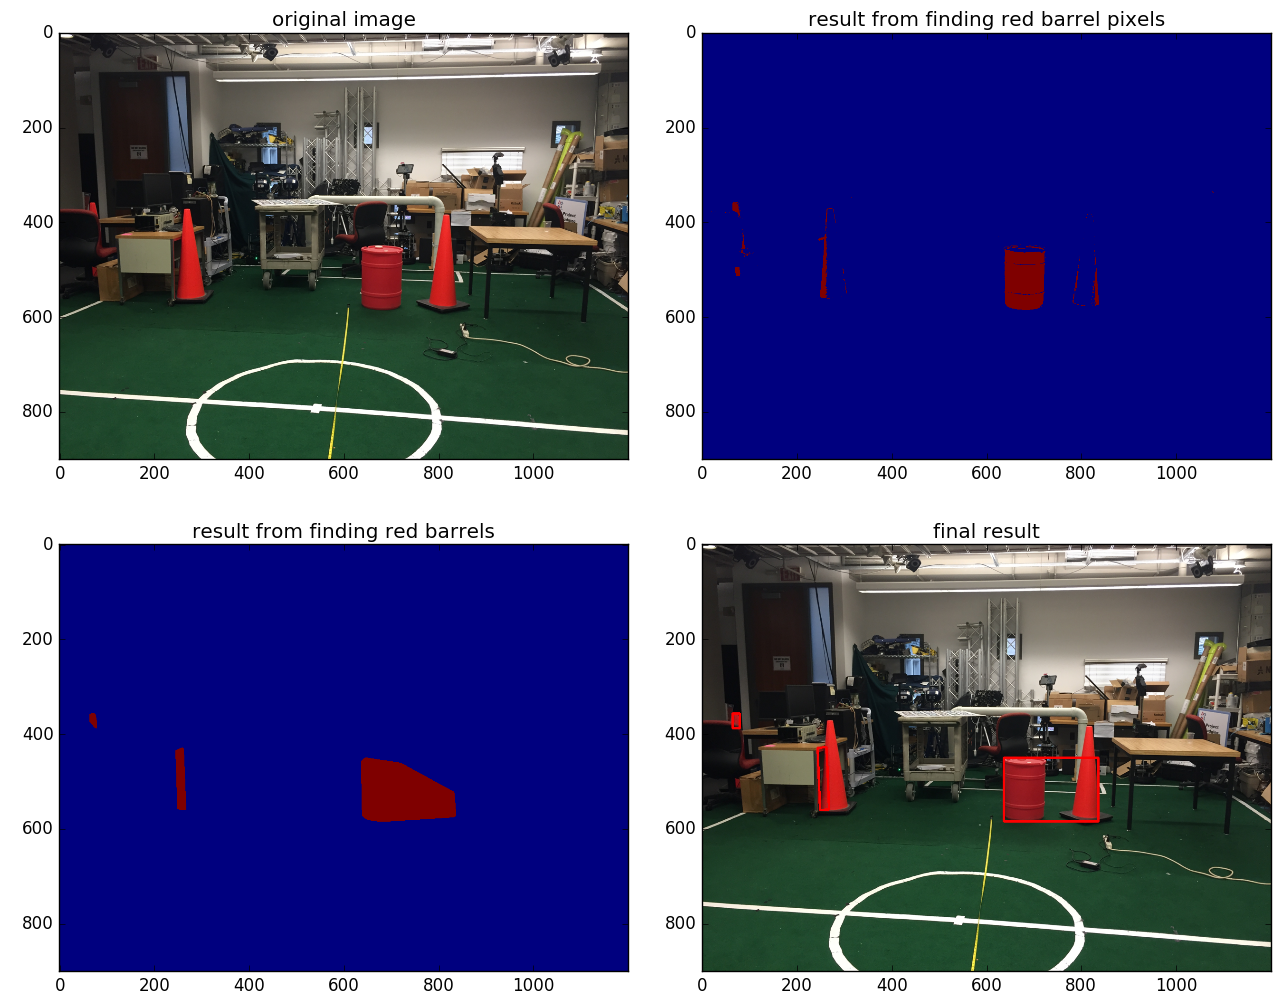
\includegraphics[scale=0.28]{result3}}}
      
      \caption{Result of a failure mode. A nearby mislabeled cone is added to the barrel and other red objects are interpreted as barrels.}
      \label{resultfig-fail}
   \end{figure}

\subsection{Test set}
Further testing was also performed on a new test set of 10 images. Detection results were very similar to those from the validation set as can be seen in Table \ref{resultstest}. One successful detection and two failure modes are shown in Figures \ref{resulttest1}, \ref{resulttest2}, and \ref{resulttest3}.
  
\begin{table}[h]
\caption{Detection results on 10 images with a total of 10 barrels. number of objects classified as barrel = 11}
\label{resultstest}
\begin{center}
\begin{tabular}{|c|c|}
\hline
detected object & \# occurences\\
\hline
full barrel & 6\\
\hline
large part of barrel & 1\\
\hline
small part of barrel & 1\\
\hline
barrel combined with non-barrel & 2\\
\hline
non-barrel & 1\\
\hline
\end{tabular}
\end{center}
\end{table}

   \begin{figure}[thpb]
      \centering
      \framebox{\parbox{3in}{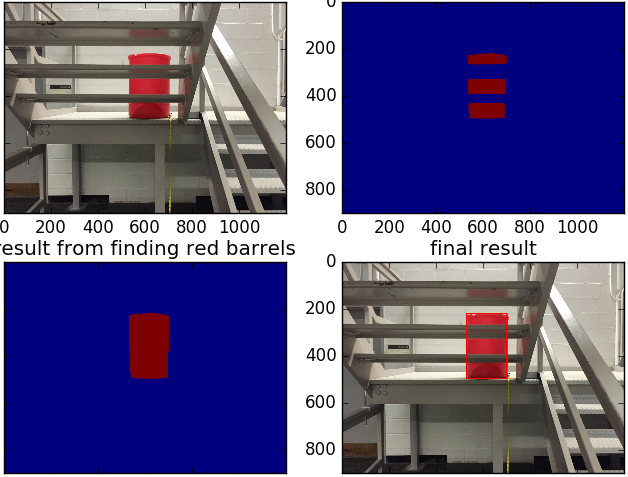
\includegraphics[scale=0.53]{result11}}}
      
      \caption{Result of a successful detection of the partially occluded red barrel.}
      \label{resulttest1}
   \end{figure}

   \begin{figure}[thpb]
      \centering
      \framebox{\parbox{3in}{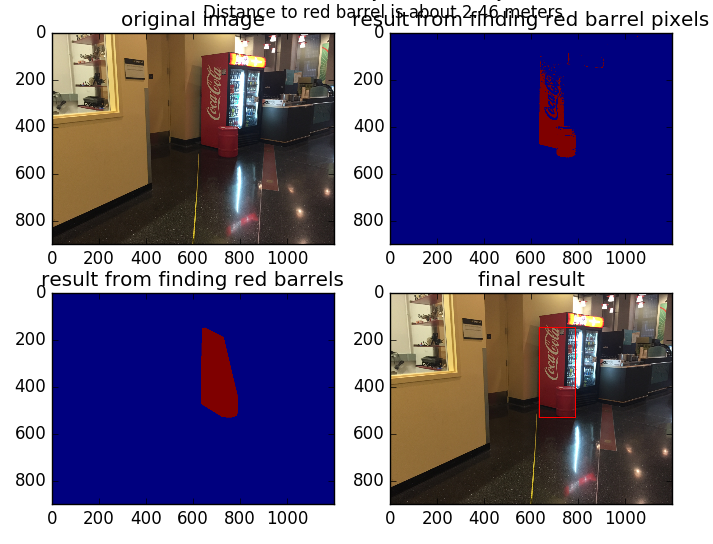
\includegraphics[scale=0.53]{result13}}}
      
      \caption{Failure mode. The red fridge has similar shape and color as a red barrel.}
      \label{resulttest2}
   \end{figure}
   
   
   \begin{figure}[thpb]
      \centering
      \framebox{\parbox{3in}{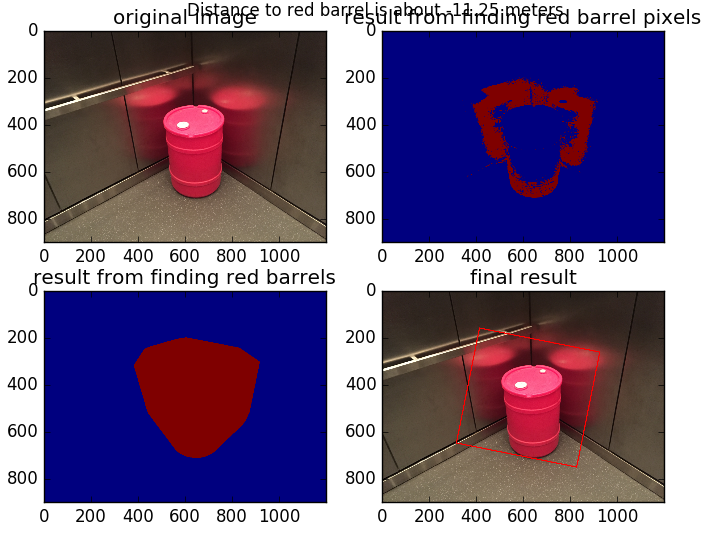
\includegraphics[scale=0.53]{result12}}}
      
      \caption{Failure mode. Oddly enough, the reflections are considered barrel red, but the barrel itself isn't. This is due to the high brightness of the barrel.}
      \label{resulttest3}
   \end{figure}
   
The coordinates of the bounding box edges in the image coordinate system are as in Table \ref{boundingboxes}.
\begin{table}[h]
\caption{Pixel coordinates of the boundingboxes and distance to barrel. The origin is on the top left of the image. The first element of each tuple represents the coordinate along the vertical axis.}
\label{boundingboxes}
\begin{center}
\begin{tabular}{|c|c|c|}
\hline
Im & box vertices & dist[m]\\
\hline
001 & [565, 520],
       [565, 378],
       [659, 378],
       [659, 520] & 5.6\\
002 & [586, 529],
       [586, 470],
       [641, 470],
       [641, 529] & 6.3\\
003 & [632, 532],
       [632, 151],
       [787, 151],
       [787, 532] & 2.5\\
004 & [636, 631],
       [461, 369],
       [627, 257],
       [802, 519] & 2.2\\
005 & [614, 514],
       [614, 457],
       [677, 457],
       [677, 514] & 6.3\\
006 & [825, 751],
       [315, 649],
       [413, 161],
       [923, 263] & 0\\
007 & [607, 187],
       [607, 112],
       [652, 112],
       [652, 187] & 6.3\\
008 & [529, 498],
       [529, 222],
       [699, 222],
       [699, 498] & 3.3\\
009 & [630, 669],
       [630, 570],
       [688, 570],
       [688, 669] & 6.1\\
010 & [629, 297],
       [629, 240],
       [668, 240],
       [668, 297] & 6.4\\
\hline     
\end{tabular}
\end{center}
\end{table}

The misclassified barrels generally had very large or very small areas which led to unbalanced relations between area and distance in the training the model. Outlier removal manually or automatically could improve results.

\section{DISCUSSION}
Instead of using a single Gaussian distribution for each color model, a Gaussian Mixture Model (GMM) can be used to better describe a color considering the different lighting conditions. As results were good and fairly invariant on the lighting conditions, this was not implemented. A simpler method would be to perform low level brightness equalization on the images. Furthermore, a robot often has multiple sequential images of the scene and can use images from different perspectives to determine if a particular object is in fact a barrel or just an artifact. Combining the likelihood of a potential barrel from the segmentation and  shape analysis may provide a metric that indicates the certainty of the detection given sequential images from the scene.

Performing analysis on the 'other red' segmented pixels may provide a way to recover false negatives. However, these additions come at the cost of oftentimes scarce computation resources and a simpler model, following Occam's razor, can avoid overfitting for unseen data. Other methods include training neural networks, but these are computationally heavy and require large training sets.



\addtolength{\textheight}{-12cm}   % This command serves to balance the column lengths
                                  % on the last page of the document manually. It shortens
                                  % the textheight of the last page by a suitable amount.
                                  % This command does not take effect until the next page
                                  % so it should come on the page before the last. Make
                                  % sure that you do not shorten the textheight too much.

%%%%%%%%%%%%%%%%%%%%%%%%%%%%%%%%%%%%%%%%%%%%%%%%%%%%%%%%%%%%%%%%%%%%%%%%%%%%%%%%



%%%%%%%%%%%%%%%%%%%%%%%%%%%%%%%%%%%%%%%%%%%%%%%%%%%%%%%%%%%%%%%%%%%%%%%%%%%%%%%%



%%%%%%%%%%%%%%%%%%%%%%%%%%%%%%%%%%%%%%%%%%%%%%%%%%%%%%%%%%%%%%%%%%%%%%%%%%%%%%%%


%%%%%%%%%%%%%%%%%%%%%%%%%%%%%%%%%%%%%%%%%%%%%%%%%%%%%%%%%%%%%%%%%%%%%%%%%%%%%%%%


\end{document}
